% Baccalauréat malgache, série C, 2009 : corrigé.
\TCDBacAttribution{C}{2009}
\providecommand{\cm}{~\mathrm{cm}}
\providecommand{\Plan}{(\mathscr{P})}
\providecommand{\dx}{~\mathrm{d}x}
\providecommand{\dt}{\mathrm{d}t}
\providecommand{\Ouv}{(O;\vec{u},\vec{v})}
\providecommand{\mes}[2]{\mathrm{mes}\left( \widehat{ \overrightarrow{#1} ; \overrightarrow{#2} } \right)}
\providecommand{\D}{(\mathscr{D})}
\providecommand{\Courbe}{(\mathscr{C})}
\providecommand{\Courben}{(\mathscr{C}_n)}
\providecommand{\CourbeU}{(\mathscr{C}_1)}
\providecommand{\CourbeD}{(\mathscr{C}_2)}
\providecommand{\bary}[1]{\mathrm{bar}\left\lbrace #1 \right\rbrace}
\providecommand{\congru}[3]{#1 \equiv #2 \quad \left[ \mathrm{mod}~#3\right]}
\providecommand{\Angl}[2]{\left( \widehat{ \overrightarrow{#1} , \overrightarrow{#2} } \right)}
%
%%%%%%%%%%%%%%%%%%%%%%%%%%%%%%%%%%%%%%%%%%%%%%%%%%%%%%%%%%%%%%%%%%%%%%%%%%%%%%%%%%%%%%%%%%%%%%%%%%%%%%%%%%%%%%%%%%%%%%%%%%%%%%%%
\noindent \underline{\textsc{\textbf{Exercice}}} (4 points)
\begin{description}
	\item[A- Probabilité :]
	Les six faces portent les lettres F, L, E, U, R, S : quatre consonnes (F, L, R, S) et deux voyelles (E, U).
	Un « mot » est une suite de trois lettres ; les lancers étant indépendants et le dé équilibré, les $6^3 = 216$ mots sont équiprobables.
	\begin{enumerate}
		\item
		\begin{itemize}
			\item \vln{Événement $A$ :}
				$4$ choix pour la première lettre, $6$ pour chacune des deux autres : $4 \times 6 \times 6 = 144$ mots.
				$P(A) = \frac{144}{216}$, soit \par\noindent\ansbox{$P(A) = \frac{2}{3}$.}
			\item \vln{Événement $B$ :}
				La troisième lettre est imposée par la première : $6 \times 6 \times 1 = 36$ mots.
				$P(B) = \frac{36}{216}$, soit \par\noindent\ansbox{$P(B) = \frac{1}{6}$.}
		\end{itemize}
		\item
		\begin{enumerate}
			\item \vln{Événement contraire :}
				\ansbox{$\overline{C}$ : « le mot obtenu contient au moins deux lettres identiques ».}
			\item \vln{Probabilité de $\overline{C}$ :}
				Les mots à lettres toutes différentes sont des arrangements : $6 \times 5 \times 4 = 120$, donc $P(C) = \frac{120}{216} = \frac{5}{9}$.
				$P(\overline{C}) = 1 - \frac{5}{9}$, soit \par\noindent\ansbox{$P(\overline{C}) = \frac{4}{9}$.}
		\end{enumerate}
	\end{enumerate}
	\item[B- Arithmétique :]
	\begin{enumerate}
		\item \vln{Calcul dans $\mathbb{Z}/6\mathbb{Z}$ :}
			Pour $a = \dot{4}$ : $a^2 + \dot{3}a + \dot{2} = \dot{16} + \dot{12} + \dot{2} = \dot{30}$, et $30 = 5 \times 6$.
			\par\noindent\ansbox{$a^2 + \dot{3}a + \dot{2} = \dot{0}$ pour $a = \dot{4}$.}
			(En effet $a^2 + 3a + 2 = (a+1)(a+2)$ et $5 \times 6 = 30$.)
		\item
		\begin{enumerate}
			\item \vln{Résolution de $(E)$ :}
				$7x = 3y$, donc $3$ divise $7x$ ; comme $\pgcd{3}{7} = 1$, $3$ divise $x$ (Gauss) : $x = 3k$, $k \in \mathbb{Z}$, puis $7 \times 3k = 3y$, d'où $y = 7k$.
				Réciproquement $7(3k) - 3(7k) = 0$.
				\par\noindent\ansbox{Les solutions de $(E)$ sont les couples $(3k \, ; 7k)$, $k \in \mathbb{Z}$.}
			\item \vln{Solution particulière et résolution de (F) :}
				Algorithme d'Euclide : $7 = 2 \times 3 + 1$, donc $1 = 7 \times 1 - 3 \times 2$. En multipliant par $2$ : $7 \times 2 - 3 \times 4 = 2$.
				\par\noindent\ansbox{$(2 \, ; 4)$ est une solution particulière de (F).}
				Si $(x,y)$ est solution de (F), alors $7(x - 2) - 3(y - 4) = 0$ : $(x - 2 \, ; y - 4)$ est solution de $(E)$, donc $x - 2 = 3k$ et $y - 4 = 7k$.
				Réciproquement ces couples conviennent.
				\par\noindent\ansbox{Les solutions de (F) sont les couples $(2 + 3k \, ; 4 + 7k)$, $k \in \mathbb{Z}$.}
		\end{enumerate}
	\end{enumerate}
\end{description}
%%%%%%%%%%%%%%%%%%%%%%%%%%%%%%%%%%%%%%%%%%%%%%%%%%%%%%%%%%%%%%%%%%%%%%%%%%%%%%%%%%%%%%%%%%%%%%%%%%%%%%%%%%%%%%%%%%%%%%%%%%%%%%%%
\noindent \underline{\textsc{\textbf{PROBLEME I}}} (7 points)
\begin{description}
	\item[Partie A]
	\vln{Construction :}
	$D$ est l'image de $C$ par la rotation $r$ de centre $O$ et d'angle $\frac{\pi}{2}$ ; $A$ est l'image de $E$ par $r$, donc $E$ est l'image de $A$ par la rotation de centre $O$ et d'angle $-\frac{\pi}{2}$.
	\begin{center}
	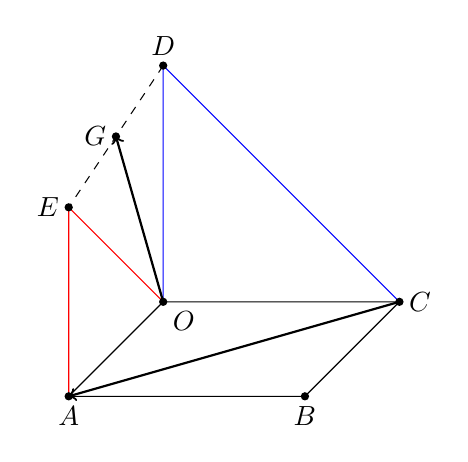
\begin{tikzpicture}[scale=.6]
		\coordinate (A) at (-1,0); \coordinate (B) at (4,0); \coordinate (C) at (6,2); \coordinate (O) at (1,2);
		\coordinate (D) at (1,7); \coordinate (E) at (-1,4); \coordinate (G) at (0,5.5);
		\draw (O) -- (A) -- (B) -- (C) -- cycle;
		\draw[blue] (O) -- (D) -- (C);
		\draw[red] (O) -- (E) -- (A);
		\draw[dashed] (D) -- (E);
		\draw[thick,->] (O) -- (G);
		\draw[thick,->] (C) -- (A);
		\foreach \P/\pos in {A/below,B/below,C/right,O/below right,D/above,E/left,G/left}
			\fill (\P) circle (2.5pt) node[\pos] {$\P$};
	\end{tikzpicture}
	\end{center}
	\item[Partie B]
	\begin{enumerate}
		\item \textbf{Par les nombres complexes.}
			(Pour utiliser les nombres complexes, le repère d'origine $O$ doit être orthonormé direct ; l'énoncé dit « orthogonal », il faut lire « orthonormé ».)
		\begin{enumerate}
			\item \vln{Affixes de $D$ et $A$ :}
				La rotation $r$ de centre $O$ et d'angle $\frac{\pi}{2}$ s'écrit $z' = iz$. Comme $D = r(C)$ et $A = r(E)$ :
				\par\noindent\ansbox{$z_D = ia$ et $z_A = ib$.}
			\item \vln{Affixes $Z$ et $Z'$ :}
				$Z = z_A - z_C$ et $Z' = z_G - z_O = \frac{z_D + z_E}{2}$ :
				\par\noindent\ansbox{$Z = ib - a$ et $Z' = \frac{ia + b}{2}$.}
			\item \vln{Relation entre $Z'$ et $Z$ :}
				$Z = ib - a = i(b + ia) = 2i \cdot \frac{ia + b}{2} = 2iZ'$, d'où \par\noindent\ansbox{$Z' = -\frac{i}{2}\, Z$.}
			\item \vln{Conclusion :}
				$Z = 2iZ'$ et $Z' \neq 0$ (sinon $Z = 0$ et $A = C$, impossible pour les sommets opposés d'un parallélogramme) : $\frac{Z}{Z'} = 2i$ est imaginaire pur, donc $\Angl{OG}{CA} = \arg(2i) = \frac{\pi}{2}$ ; et $|Z| = 2|Z'|$.
				\par\noindent\ansbox{$\overrightarrow{CA} \perp \overrightarrow{OG}$ et $CA = 2\,OG$.}
		\end{enumerate}
		\item \textbf{Par les transformations.}
		\begin{enumerate}
			\item \vln{Nature de $s$ :}
				$r$ est une similitude directe de rapport $1$ et d'angle $\frac{\pi}{2}$, $h$ est une similitude directe de rapport $2$ et d'angle $0$.
				\par\noindent\ansbox{$s = r \circ h$ est une similitude directe de rapport $2$ et d'angle $\frac{\pi}{2}$.}
			\item \vln{$s(G)$ et $s(O)$ :}
				$G$ est le milieu de $[DE]$, donc $\overrightarrow{DE} = 2\overrightarrow{DG}$ : $h(G) = E$ ; puis $r(E) = A$. Donc $s(G) = A$.
				$h(O) = O_1$ avec $\overrightarrow{DO_1} = 2\overrightarrow{DO}$ : $O$ est le milieu de $[DO_1]$, donc $O_1 = \sigma_O(D)$ où $\sigma_O$ est la symétrie de centre $O$.
				Or $r \circ r = \sigma_O$ (deux quarts de tour) et $r$ commute avec $\sigma_O$ ; comme $D = r(C)$ :
				$r(O_1) = r \circ \sigma_O \circ r (C) = \sigma_O \circ (r \circ r)(C) = \sigma_O \circ \sigma_O (C) = C$.
				\par\noindent\ansbox{$s(G) = A$ et $s(O) = C$.}
			\item \vln{Conclusion :}
				La similitude directe $s$ transforme le segment $[OG]$ en $[CA]$ : $CA = 2\,OG$ (rapport $2$) et
				$\Angl{OG}{CA} = \frac{\pi}{2}$ (angle de $s$).
				\par\noindent\ansbox{$\overrightarrow{CA} \perp \overrightarrow{OG}$ et $CA = 2\,OG$.}
		\end{enumerate}
	\end{enumerate}
	\item[Partie C]
	Les vecteurs $\overrightarrow{OC}$ et $\overrightarrow{OD}$ sont orthogonaux, de même longueur et $\Angl{OC}{OD} = \frac{\pi}{2}$ : le repère $(O;\overrightarrow{OC},\overrightarrow{OD})$ est orthonormé direct, avec $z_C = 1$ et $z_D = i$.
	\begin{itemize}
		\item $h : z' - i = 2(z - i)$, soit $z' = 2z - i$ ;
		\item $r : z' = iz$ ;
		\item $s = r \circ h : z' = i(2z - i) = 2iz + 1$.
	\end{itemize}
	\ansbox{$s : z' = 2iz + 1$.}
	Le centre $\Omega$ vérifie $\omega = 2i\omega + 1$, d'où $\omega = \frac{1}{1 - 2i} = \frac{1 + 2i}{5}$.
	\par\noindent\ansbox{Le centre de $s$ a pour affixe $\frac{1}{5} + \frac{2}{5} i$.}
	(Vérification : $s(0) = 1 = z_C$.)
\end{description}
%%%%%%%%%%%%%%%%%%%%%%%%%%%%%%%%%%%%%%%%%%%%%%%%%%%%%%%%%%%%%%%%%%%%%%%%%%%%%%%%%%%%%%%%%%%%%%%%%%%%%%%%%%%%%%%%%%%%%%%%%%%%%%%%
\noindent \underline{\textsc{\textbf{PROBLEME II}}} (9 points)
\begin{description}
	\item[Partie A]
	\begin{enumerate}
		\item
		\begin{enumerate}
			\item \vln{Tableau de variation de $g$ :}
				$g'(x) = -(2x - 2)\expo{-x} + (x^2 - 2x + 2)\expo{-x} = (x^2 - 4x + 4)\expo{-x} = (x-2)^2\expo{-x} \geq 0$,
				nul seulement en $2$ : $g$ est strictement croissante sur $\mathbb{R}$.
				En $-\infty$ : $x^2 - 2x + 2 \to +\infty$ et $\expo{-x} \to +\infty$, donc $g(x) \to -\infty$.
				En $+\infty$ : $(x^2 - 2x + 2)\expo{-x} = \frac{x^2}{\expo{x}} - \frac{2x}{\expo{x}} + \frac{2}{\expo{x}} \to 0$, donc $g(x) \to 1$.
				\[
				\begin{array}{c|ccccc}
					x & -\infty & & 2 & & +\infty \\ \hline
					g'(x) & & + & 0 & + & \\ \hline
					 & & & & & 1 \\
					g & & \nearrow & 1 - 2\expo{-2} & \nearrow & \\
					 & -\infty & & & &
				\end{array}
				\]
			\item \vln{Solution unique $\alpha$ :}
				$g$ est continue et strictement croissante de $\mathbb{R}$ sur $]-\infty ; 1[$, qui contient $0$ : l'équation $g(x) = 0$ a une unique solution $\alpha$.
				$g(0{,}35) \approx -0{,}0024 < 0$ et $g(0{,}36) \approx 0{,}0166 > 0$, donc
				\par\noindent\ansbox{$0{,}35 \leq \alpha \leq 0{,}36$ (en fait $\alpha \approx 0{,}3513$).}
			\item \vln{Signe de $g$ :}
				\ansbox{$g(x) < 0$ pour $x < \alpha$, $g(\alpha) = 0$, $g(x) > 0$ pour $x > \alpha$.}
		\end{enumerate}
		\item
		\begin{enumerate}
			\item \vln{$f' = g$ :}
				$f'(x) = 1 + 2x\expo{-x} - (x^2 + 2)\expo{-x} = 1 - (x^2 - 2x + 2)\expo{-x}$.
				\par\noindent\ansbox{$f'(x) = g(x)$ pour tout réel $x$.}
			\item \vln{Tableau de variation de $f$ :}
				En $-\infty$ : $(x^2 + 2)\expo{-x} \to +\infty$ l'emporte sur $x - 1$ : en écrivant $f(x) = x^2\expo{-x}\left(\frac{x - 1}{x^2\expo{-x}} + 1 + \frac{2}{x^2}\right)$
				et $\frac{x-1}{x^2\expo{-x}} \to 0$, on obtient $f(x) \to +\infty$.
				En $+\infty$ : $(x^2+2)\expo{-x} \to 0$ et $x - 1 \to +\infty$, donc $f(x) \to +\infty$.
				Le minimum est $f(\alpha) \approx 0{,}85$ (avec $\alpha = 0{,}35$ : $f(0{,}35) \approx 0{,}85$).
				\[
				\begin{array}{c|ccccc}
					x & -\infty & & \alpha & & +\infty \\ \hline
					f'(x) & & - & 0 & + & \\ \hline
					 & +\infty & & & & +\infty \\
					f & & \searrow & & \nearrow & \\
					 & & & f(\alpha) \approx 0{,}85 & &
				\end{array}
				\]
			\item \vln{Asymptote $\D$ :}
				$f(x) - (x - 1) = (x^2 + 2)\expo{-x} = \frac{x^2}{\expo{x}} + \frac{2}{\expo{x}} \to 0$ quand $x \to +\infty$.
				\par\noindent\ansbox{$\D : y = x - 1$ est asymptote à $\Courbe$ en $+\infty$,}
				et $\Courbe$ est au-dessus de $\D$ car $(x^2+2)\expo{-x} > 0$.
				En $-\infty$, $\frac{f(x)}{x} \to -\infty$ : $\Courbe$ a une branche parabolique de direction $(Oy)$.
			\item \vln{Tracé (figure réduite, unité $1{,}5\cm$) :}
				Valeurs : $f(-0{,}5) \approx 2{,}21$ ; $f(0) = 1$ ; $f(1) \approx 1{,}10$ ; $f(2) \approx 1{,}81$ ; $f(3) \approx 2{,}55$ ; $f(4) \approx 3{,}33$.
				\begin{center}
				\begin{tikzpicture}[x=1.5cm,y=1.5cm,>=stealth]
					\draw[->] (-1.2,0) -- (5,0) node[below] {$x$};
					\draw[->] (0,-1.5) -- (0,4.2) node[left] {$y$};
					\foreach \t in {-1,1,2,3,4} \draw (\t,0.03) -- (\t,-0.03) node[below] {\small $\t$};
					\foreach \t in {1,2,3,4} \draw (0.03,\t) -- (-0.03,\t) node[left] {\small $\t$};
					\node[below left] at (0,0) {$O$};
					\draw[red] (-0.5,-1.5) -- (4.8,3.8) node[right] {$\D$};
					\draw[blue,thick] plot[domain=-0.8:4.8,samples=120] (\x,{\x-1+(\x*\x+2)*exp(-\x)});
					\draw[dashed] (0.35,0) node[below] {\small $\alpha$} -- (0.35,0.846);
					\node[blue] at (-0.5,3.3) {$\Courbe$};
				\end{tikzpicture}
				\end{center}
		\end{enumerate}
	\end{enumerate}
	\item[Partie B]
	\begin{enumerate}
		\item
		\begin{enumerate}
			\item \vln{$h$ est strictement décroissante sur $I$ :}
				$h'(x) = f'(x) - 1 = g(x) - 1 = -(x^2 - 2x + 2)\expo{-x}$.
				Or $x^2 - 2x + 2 = (x-1)^2 + 1 > 0$, donc $h'(x) < 0$ : $h$ est strictement décroissante sur $I$.
				$h(1) = f(1) - 1 = \frac{3}{\expo{1}} - 1 \approx 0{,}10$ et $h(2) = f(2) - 2 = \frac{6}{\expo{2}} - 1 \approx -0{,}19$.
				\[
				\begin{array}{c|ccc}
					x & 1 & & 2 \\ \hline
					h'(x) & & - & \\ \hline
					 & \frac{3}{e} - 1 & & \\
					h & & \searrow & \\
					 & & & \frac{6}{e^2} - 1
				\end{array}
				\]
			\item \vln{Solution unique $\beta$ :}
				$h$ est continue, strictement décroissante sur $I$, avec $h(1) > 0 > h(2)$ : $h(x) = 0$, c'est-à-dire $f(x) = x$, a une unique solution dans $I$.
				\par\noindent\ansbox{L'équation $f(x) = x$ a une unique solution $\beta \in [1;2]$ (en fait $\beta \approx 1{,}319$).}
		\end{enumerate}
		\item \vln{$f(I) \subset I$ et $|f'| \leq \frac{3}{4}$ sur $I$ :}
			Sur $I$, $x > \alpha$ donc $f$ est croissante : $f(I) = [f(1) ; f(2)] = \left[\frac{3}{e} ; 1 + \frac{6}{e^2}\right] \approx [1{,}10 ; 1{,}81] \subset [1;2]$.
			$f' = g$ est croissante et positive sur $I$ : $0 < g(1) \leq f'(x) \leq g(2) = 1 - \frac{2}{e^2}$.
			Or $1 - \frac{2}{e^2} \leq \frac{3}{4} \iff \frac{2}{e^2} \geq \frac{1}{4} \iff e^2 \leq 8$, vrai car $e^2 \approx 7{,}39$.
			\par\noindent\ansbox{Pour $x \in I$ : $f(x) \in I$ et $|f'(x)| \leq \frac{3}{4}$.}
		\item
		\begin{enumerate}
			\item \vln{$U_n \in I$ :}
				$U_0 = 1 \in I$ ; si $U_n \in I$, alors $U_{n+1} = f(U_n) \in I$ d'après 2.
				\par\noindent\ansbox{Pour tout $n \in \mathbb{N}$, $U_n \in I$.}
			\item \vln{Inégalités :}
				$U_n$ et $\beta$ sont dans $I$ où $|f'| \leq \frac{3}{4}$ ; l'inégalité des accroissements finis donne
				$|f(U_n) - f(\beta)| \leq \frac{3}{4}|U_n - \beta|$, et $f(U_n) = U_{n+1}$, $f(\beta) = \beta$ :
				\par\noindent\ansbox{$|U_{n+1} - \beta| \leq \frac{3}{4}|U_n - \beta|$.}
				Par récurrence immédiate (vrai pour $n = 0$ ; on multiplie par $\frac{3}{4}$ pour passer de $n$ à $n+1$) :
				\par\noindent\ansbox{$|U_n - \beta| \leq \left(\frac{3}{4}\right)^n |U_0 - \beta|$.}
			\item \vln{Convergence :}
				$0 < \frac{3}{4} < 1$ donc $\left(\frac{3}{4}\right)^n \to 0$ et $|U_n - \beta| \to 0$.
				\par\noindent\ansbox{$(U_n)$ converge vers $\ell = \beta$.}
		\end{enumerate}
		\item \vln{Entier $p$ :}
			$U_0 = 1$ et $\beta \in [1;2]$, donc $|U_0 - \beta| \leq 1$ et $|U_n - \beta| \leq \left(\frac{3}{4}\right)^n$.
			Il suffit que $\left(\frac{3}{4}\right)^n \leq 10^{-2}$, c'est-à-dire $n \ln\frac{3}{4} \leq -2\ln 10$, soit
			$n \geq \frac{2\ln 10}{\ln\frac{4}{3}} \approx 16{,}01$.
			Comme $\left(\frac{3}{4}\right)^n$ décroît, \par\noindent\ansbox{$p = 17$ convient : pour $n \geq 17$, $|U_n - \beta| \leq 10^{-2}$.}
			(C'est le plus petit entier que donne cette majoration ; une estimation plus fine de $\beta - 1$ donnerait un $p$ plus petit.)
	\end{enumerate}
\end{description}
